\documentclass[../main.tex]{subfiles}
\begin{document}
    \subsection {Выборочные коэффициенты корреляции}
    \begin{table}[H]
        \centering
        \begin{tabular}{|c|c|c|c|}
            \hline
            & $r$ & $r_S$ & $r_Q$\\\hline
            $\rho=0$ & & &\\\hline
            $E(z)$ & -0.0017 & 0.0023 & 0.0\\\hline
            $E(z^2)$ & 0.0267 & 0.0249 & 0.04\\\hline
            $D(z)$ & 0.0527 & 0.0526 & 0.0482\\\hline
            \hline
            $\rho=0.5$ & & &\\\hline
            $E(z)$ & 0.5117 & 0.4767 & 0.4\\\hline
            $E(z^2)$ & 0.2618 & 0.2272 & 0.16\\\hline
            $D(z)$ & 0.0319 & 0.0348 & 0.0473\\\hline
            \hline
            $\rho=0.9$ & & &\\\hline
            $E(z)$ & 0.9094 & 0.8857 & 0.8\\\hline
            $E(z^2)$ & 0.827 & 0.7845 & 0.64\\\hline
            $D(z)$ & 0.0024 & 0.0043 & 0.0285\\\hline
        \end{tabular}
        \caption{Характеристики распределения размерностью n = 20}
    \end{table}
    
    \begin{table}[H]
        \centering
        \begin{tabular}{|c|c|c|c|}
            \hline
            & $r$ & $r_S$ & $r_Q$\\\hline
            $\rho=0$ & & &\\\hline
            $E(z)$ & 0.0039 & 0.0066 & 0.0\\\hline
            $E(z^2)$ & 0.0084 & 0.0088 & 0.0044\\\hline
            $D(z)$ & 0.0179 & 0.0181 & 0.0174\\\hline
            \hline
            $\rho=0.5$ & & &\\\hline
            $E(z)$ & 0.5002 & 0.4741 & 0.3333\\\hline
            $E(z^2)$ & 0.2502 & 0.2248 & 0.1111\\\hline
            $D(z)$ & 0.01 & 0.0111 & 0.015\\\hline
            \hline
            $\rho=0.9$ & & &\\\hline
            $E(z)$ & 0.903 & 0.8881 & 0.7333\\\hline
            $E(z^2)$ & 0.8153 & 0.7887 & 0.5378\\\hline
            $D(z)$ & 0.0007 & 0.0011 & 0.0087\\\hline
        \end{tabular}
        \caption{Характеристики распределения размерностью n = 60}
    \end{table}
    
    \begin{table}[H]
        \centering
        \begin{tabular}{|c|c|c|c|}
            \hline
            & $r$ & $r_S$ & $r_Q$\\\hline
            $\rho=0$ & & &\\\hline
            $E(z)$ & -0.0007 & -0.0014 & 0.0\\\hline
            $E(z^2)$ & 0.0049 & 0.0049 & 0.0064\\\hline
            $D(z)$ & 0.0106 & 0.0102 & 0.01\\\hline
            \hline
            $\rho=0.5$ & & &\\\hline
            $E(z)$ & 0.4999 & 0.4798 & 0.32\\\hline
            $E(z^2)$ & 0.2499 & 0.2302 & 0.1024\\\hline
            $D(z)$ & 0.0056 & 0.006 & 0.0083\\\hline
            \hline
            $\rho=0.9$ & & &\\\hline
            $E(z)$ & 0.9005 & 0.888 & 0.72\\\hline
            $E(z^2)$ & 0.8108 & 0.7885 & 0.5184\\\hline
            $D(z)$ & 0.0004 & 0.0006 & 0.0047\\\hline
        \end{tabular}
        \caption{Характеристики распределения размерностью n = 100}
    \end{table}
    
    \begin{table}[H]
        \centering
        \begin{tabular}{|c|c|c|c|}
            \hline
            & $r$ & $r_S$ & $r_Q$\\\hline
            $n=20$ & & &\\\hline
            $E(z)$ & 0.7995 & 0.7684 & 0.6\\\hline
            $E(z^2)$ & 0.6392 & 0.5905 & 0.36\\\hline
            $D(z)$ & 0.0101 & 0.0146 & 0.0373\\\hline
            \hline
            $n=60$ & & &\\\hline
            $E(z)$ & 0.7921 & 0.7723 & 0.6\\\hline
            $E(z^2)$ & 0.6275 & 0.5965 & 0.36\\\hline
            $D(z)$ & 0.0027 & 0.0038 & 0.0119\\\hline
            \hline
            $n=100$ & & &\\\hline
            $E(z)$ & 0.7918 & 0.7745 & 0.56\\\hline
            $E(z^2)$ & 0.627 & 0.5999 & 0.3136\\\hline
            $D(z)$ & 0.0015 & 0.0021 & 0.0072\\\hline
        \end{tabular}
        \caption{Смесь нормальных распределений}
    \end{table}
    
    \subsection{Эллипсы рассеивания}
    \begin{figure}[H]
        \centering
        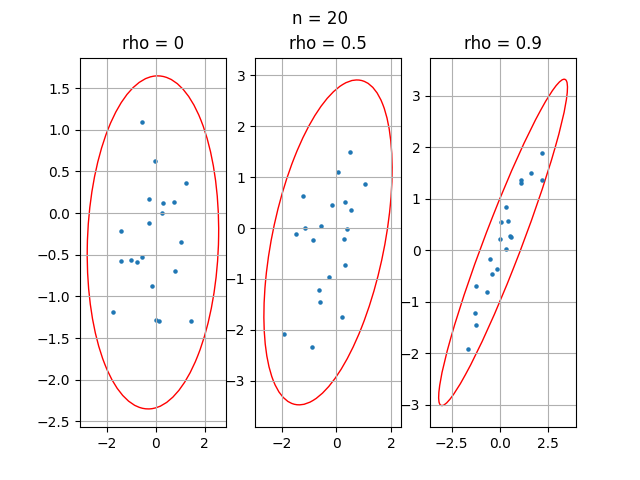
\includegraphics[scale=0.85]{figures/elipse20.png}
        \caption{Эллипс рассеивания для 20 элементов}
    \end{figure}
    
    \begin{figure}[H]
        \centering
        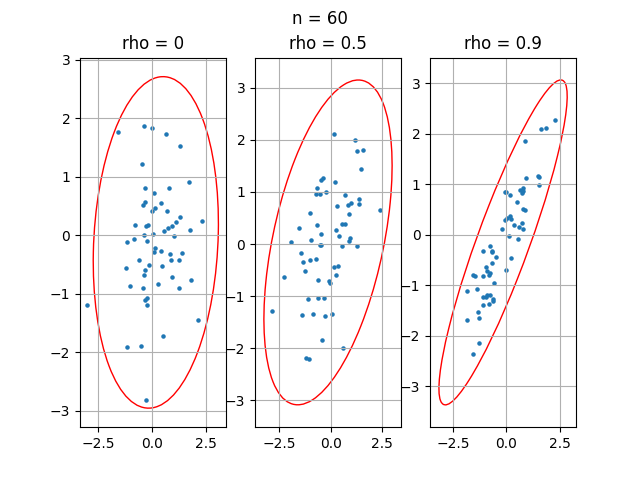
\includegraphics[scale=0.85]{figures/elipse60.png}
        \caption{Эллипс рассеивания для 60 элементов}
    \end{figure}
    
    \begin{figure}[H]
        \centering
        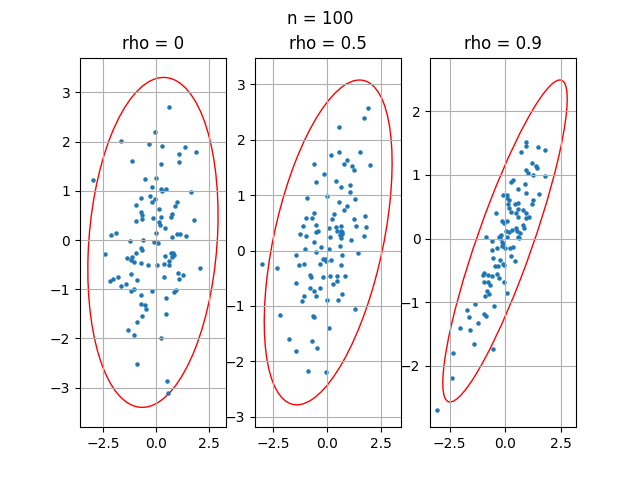
\includegraphics[scale=0.85]{figures/elipse100.png}
        \caption{Эллипс рассеивания для 100 элементов}
    \end{figure}
    
    \subsection{Оценки коэффициентов линейной регрессии}
    \subsubsection{Выборка без возмущений}
		\begin{itemize}
			\item{Критерий наименьших квадратов:}
			$\hat{a}\approx 2.26$, $\hat{b}\approx 1.77$
			\item{Критерий наименьших модулей:}
			$\hat{a}\approx 2.28$, $\hat{b}\approx 1.7$
		\end{itemize}
		\begin{figure}[H]
			\centering
			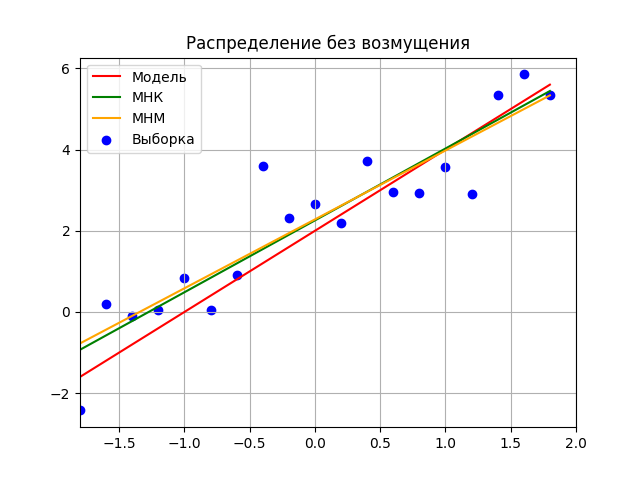
\includegraphics[width = 10cm, height 8cm]{figures/noDisturbance.png}
			\caption{Выборка без возмущений}
			\label{w/o_pert}
		\end{figure}
	
	\subsubsection{Выборка с возмущениями}
		\begin{itemize}
			\item{Критерий наименьших квадратов:}
			$\hat{a}\approx 2.26$, $\hat{b}\approx 0.19$
			\item{Критерий наименьших модулей:}
			$\hat{a}\approx 2.15$, $\hat{b}\approx 1.32$
		\end{itemize}
		\begin{figure}[H]
			\centering
			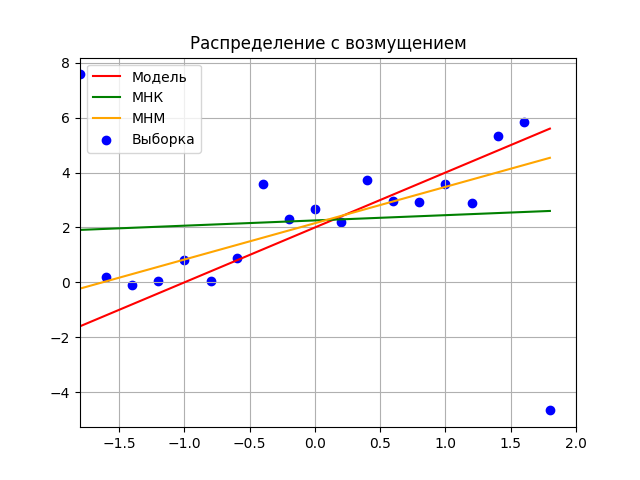
\includegraphics[width = 10cm, height = 8cm]{figures/Disturbance.png}
			\caption{Выборка с возмущениями}
			\label{w_pert}
		\end{figure}
		
		
    \subsection{Проверка гипотезы о законе распределения генеральной совокупности. Метод хи-квадрат}
    
    \noindent Метод максимального правдоподобия:
    \newline
    $\hat{\mu} \approx 0.24, \hat{\sigma} \approx 1.17$
    \newline Критерий согласия $\chi^{2}$:
    \begin{itemize}
        \item Количество промежутков $k = 8$
        \item Уровень значимости $\alpha$= 0.05
        \item Тогда квантиль $\chi^{2}_{1-\alpha}(k-1)$ = $\chi^{2}_{0.95}(7)$. Из таблицы [3, с. 358] $\chi^{2}_{0.95}(7) \approx 14.07$.
    \end{itemize}

    \newline
 
    \begin{table}[H]
    	\centering
    	\begin{tabular}{| c | c | c | c | c | c | c |}
    		\hline
    		$i$ & $limits$         &   $n_i$ &    $p_i$ &   $np_i$ &   $n_i - np_i$ &   $\frac{(n_i-np_i)^2}{np_i}$ \\
            \hline
                1 & ['-inf', -1.1]     &  12 & 0.1357 &  13.5666 & -1.5666 &  0.1809 \\
                2 & [-1.1, -0.7333]    &   6 & 0.096  &   9.6012 & -3.6012 &  1.3507 \\
                3 & [-0.7333, -0.3667] &  12 & 0.1253 &  12.5256 & -0.5256 &  0.0221 \\
                4 & [-0.3667, 0.0]     &  14 & 0.1431 &  14.3066 & -0.3066 &  0.0066 \\
                5 & [0.0, 0.3667]      &   9 & 0.1431 &  14.3066 & -5.3066 &  1.9683 \\
                6 & [0.3667, 0.7333]   &  17 & 0.1253 &  12.5256 &  4.4744 &  1.5983 \\
                7 & [0.7333, 1.1]      &   7 & 0.096  &   9.6012 & -2.6012 &  0.7047 \\
                8 & [1.1, 'inf']       &  23 & 0.1357 &  13.5666 &  9.4334 &  6.5594 \\
                9 & -                  & 100 & 1      & 100      &  0      & 12.391  \\
            \hline
    	\end{tabular}
    	\caption{ Вычисление $\chi^{2}_{B}$ при проверке гипотезы $H_{0}$ о нормальном законе распределения $N(x,\hat{\mu}, \hat{\sigma})$}
    	\label{tab:normal_chi_2}
    \end{table} 
    
    \noindent Сравнивая $\chi^{2}_{B} = 12.39$ и $\chi^{2}_{0.95}(7) \approx 14.07$, видим, что $\chi^{2}_{B} < \chi^{2}_{0.95}$.
    \\
    
    \begin{table}[H]
    	\centering
    	\begin{tabular}{| c | c | c | c | c | c | c |}
    		\hline
    		$i$ & $limits$         &   $n_i$ &    $p_i$ &   $np_i$ &   $n_i - np_i$ &   $\frac{(n_i-np_i)^2}{np_i}$ \\
            \hline
                1 & ['-inf', -1.1]    &  2 & 0.1357 &  2.7133 & -0.7133 & 0.1875 \\
                2 & [-1.1, -0.3667]   &  3 & 0.2213 &  4.4254 & -1.4254 & 0.4591 \\
                3 & [-0.3667, 0.3667] & 10 & 0.2861 &  5.7226 &  4.2774 & 3.1971 \\
                4 & [0.3667, 1.1]     &  4 & 0.2213 &  4.4254 & -0.4254 & 0.0409 \\
                5 & [1.1, 'inf']      &  1 & 0.1357 &  2.7133 & -1.7133 & 1.0819 \\
                6 & -                 & 20 & 1      & 20      &  0      & 4.9665 \\
            \hline
    	\end{tabular}
    	\caption{ Вычисление $\chi^{2}_{B}$ при проверке гипотезы $H_{0}$ о законе распределения $L(x,\hat{\mu}, \hat{\sigma})$, $n=20$}
    	\label{tab:laplace_chi_2}
    \end{table}
    
    \noindent Сравнивая $\chi^{2}_{B} =  4.97$ и $\chi^{2}_{0.95}(4) \approx 9.49$, видим, что $\chi^{2}_{B} < \chi^{2}_{0.95}$.
    \\
    
    \subsection{Доверительные интервалы для параметров нормального распределения}
    \begin{figure}[H]
		\centering
		    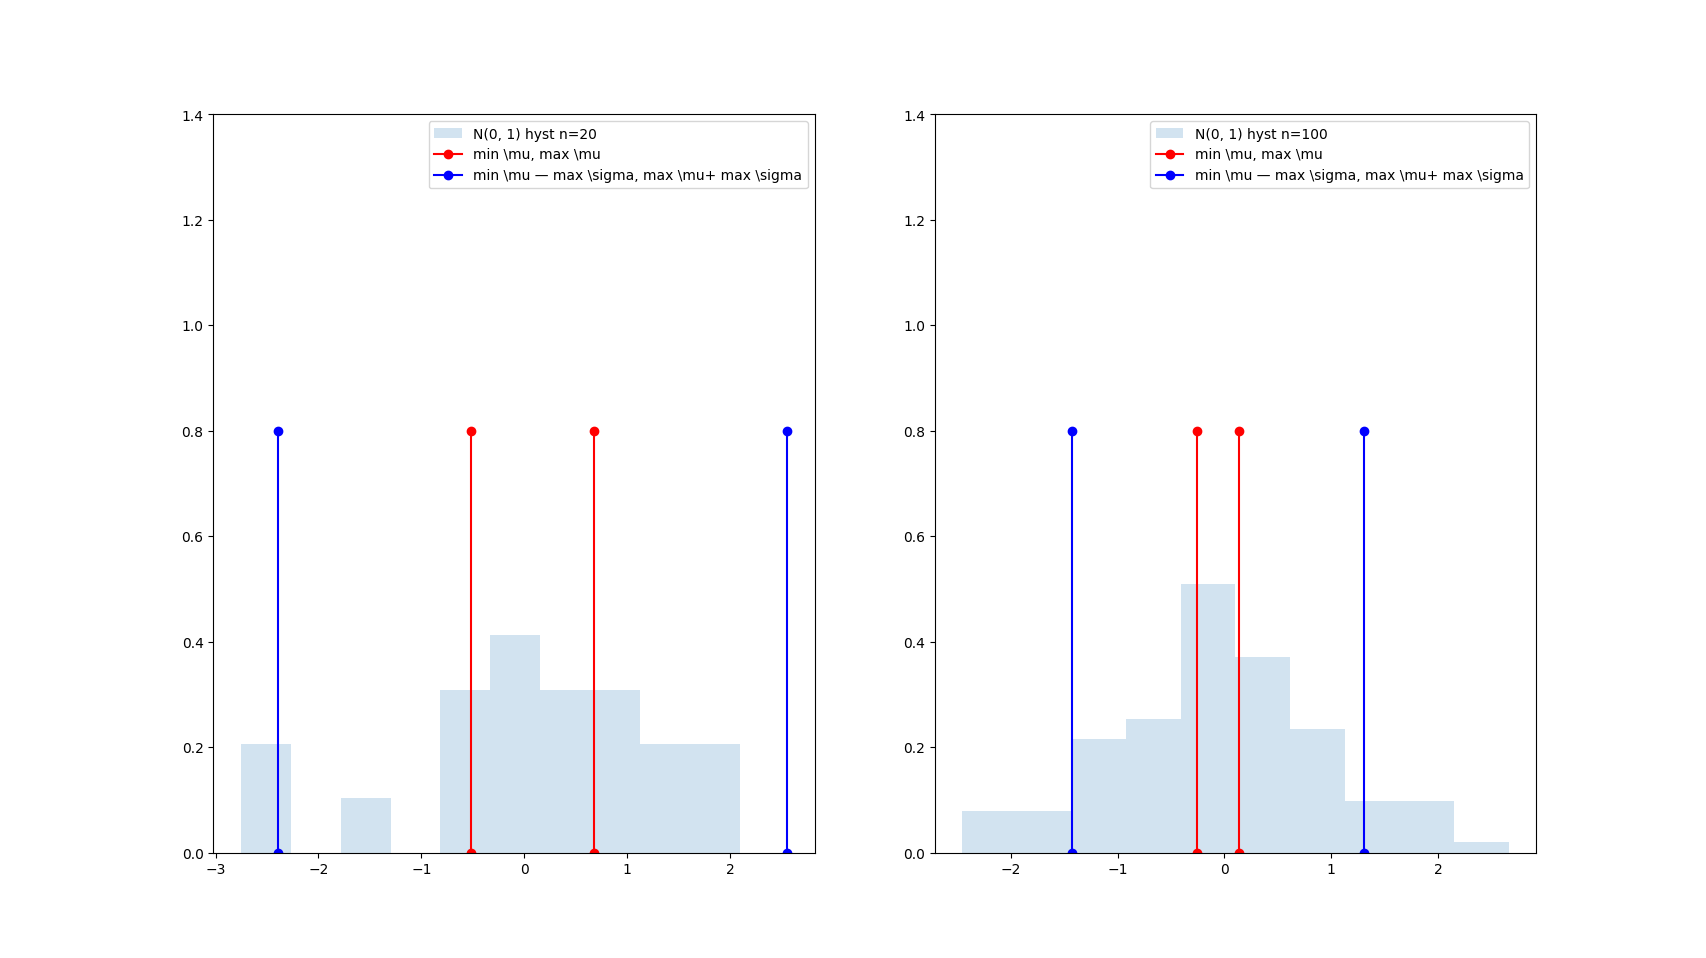
\includegraphics[width = 20cm, height = 6cm]{figures/1.png}
		\caption{Гистограммы нормальных распределений.}
		\label{w_pert}
	\end{figure}
    
	\begin{table}[H]
	    \centering
	    \begin{tabular}{| c | c | c |}
	    \hline
	       n    &  $m$  & $\sigma$\\ \hline
	        20  &  -0.29 < $m$ < 0.63 & 0.75 < $\sigma$ < 1 \\ \hline
	       100   & -0.28 < $m$ < 0.07 & 0.78 < $\sigma$ < 1 \\
	   \hline
	    \end{tabular}
	    \caption{Доверительные интервалы для параметров нормального распределения}
	    \label{tab:interv_simple}
	\end{table}
	
\subsection{Доверительные интервалы для параметров произвольного распределения. Асимптотический подход}
    \begin{figure}[H]
		\centering
			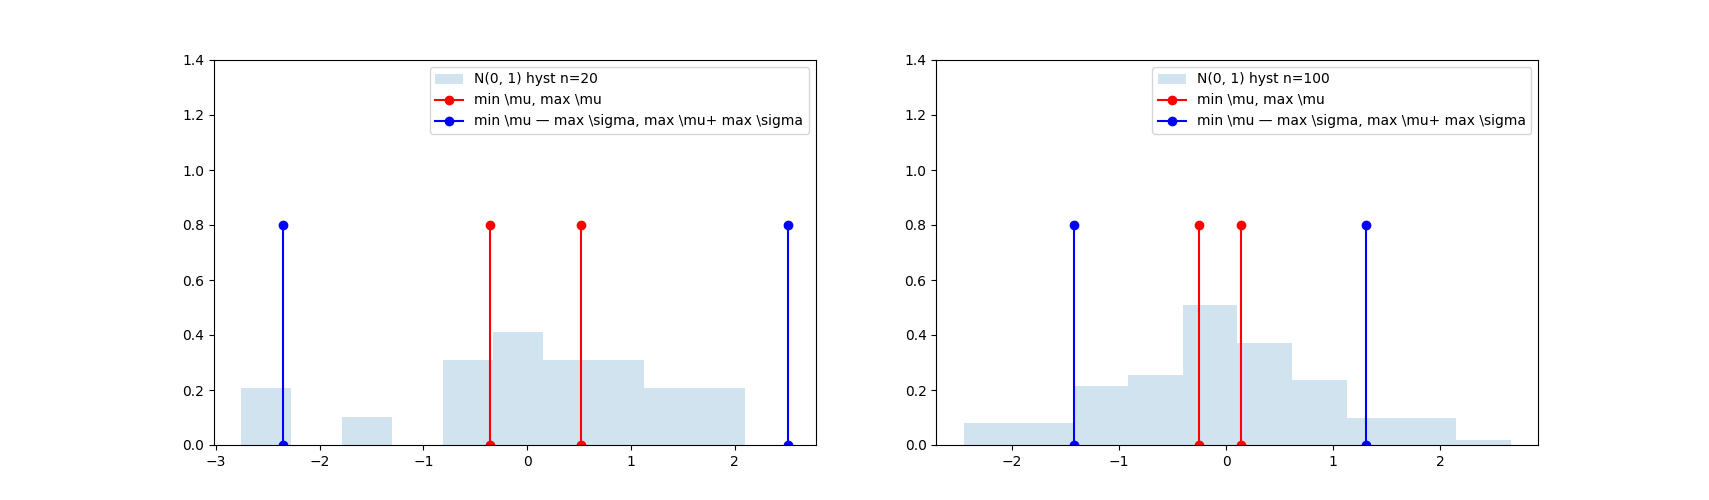
\includegraphics[width = 20cm, height = 6cm]{figures/2.png}
		\caption{Гистограммы произвольного распределения.}
		\label{w_pert}
	\end{figure}
	\begin{table}[H]
	    \centering
	    \begin{tabular}{| c | c | c |}
	    \hline
	       n    &  $m$  & $\sigma$\\ \hline
	        20  &  -0.27 < $m$ < 0.61 & 0.82 < $\sigma$ < 1.19 \\ \hline
	       100   &  -0.30 < $m$ < 0.09 & 0.80 < $\sigma$ < 0.99 \\
	   \hline
	    \end{tabular}
	    \caption{Доверительные интервалы для параметров произвольного распределения. Асимптотический подход}
	    \label{tab:interv_asimpt}
	\end{table}
\end{document}